\documentclass[11pt,a4paper]{article}

% -----------------------------------------------------------------------------
% Paquetes: todos forman parte de una instalacion estandar de LaTeX.
% -----------------------------------------------------------------------------
\usepackage[utf8]{inputenc}
\usepackage{enumitem}
\usepackage[T1]{fontenc}
% Fecha en espanol sin depender de babel ni de spanish.ldf.
\newcommand{\FechaEnEspanol}{%
  \number\day\space de\space
  \ifcase\month
    \or enero\or febrero\or marzo\or abril\or mayo\or junio\or
    julio\or agosto\or septiembre\or octubre\or noviembre\or diciembre
  \fi\space de\space\number\year
}
\usepackage[a4paper,margin=2.5cm,headheight=42pt]{geometry}
\usepackage{graphicx}
\usepackage{xcolor}
\usepackage{fancyhdr}

% lastpage no es necesario para compilar, pero permite mostrar "pagina de N".
\newif\ifHayUltimaPagina
\IfFileExists{lastpage.sty}{
  \usepackage{lastpage}
  \HayUltimaPaginatrue
}{
  \HayUltimaPaginafalse
}

% -----------------------------------------------------------------------------
% CONFIGURACION DEL TRABAJO: editar solamente este bloque para reutilizarlo.
% -----------------------------------------------------------------------------
\newcommand{\NombreMateria}{Redes de Computadoras}
\newcommand{\TipoTrabajo}{Trabajo Práctico}
\newcommand{\NumeroTrabajo}{3}
% Cambiar por "Teórico" o "Práctico" según corresponda.
\newcommand{\TipoTP}{Práctico}
\newcommand{\NombreTrabajo}{Enlace de Datos, Red y Transporte}
\newcommand{\NombreGrupo}{NetRunners}
\newcommand{\Docente}{SANTIAGO MARTIN HENN}
\newcommand{\LogoArchivo}{logo.png}
\newcommand{\LogoRuta}{\LogoArchivo}

% Una linea por integrante. Se pueden agregar o quitar filas.
\newcommand{\Integrantes}{%
  \begin{tabular}{ll}
    Bastida, Lucas Ramiro & DNI 39444511 \\
    Contessi, Ruben Andres & DNI 33315235 \\
    Garay, Ignacio Hernan & DNI 44191925 \\
    Giraudo, Juan Pablo & DNI 34970089 \\
    Peñaloza, Gonzalo Adrian & DNI 40441355 \\
    Quinteros del Castillo, Tomás Agustín & DNI 46169739 \\
    Vasconsellos Blason, Benjamin Alejandro & DNI 45642879 \\
  \end{tabular}%
}

% -----------------------------------------------------------------------------
% Elementos comunes de caratula y encabezado.
% -----------------------------------------------------------------------------
\newcommand{\InsertarLogo}[1][0.24\textwidth]{%
  \ifx\LogoRuta\empty
    \fbox{\parbox[c][1cm][c]{#1}{\centering Logo institucional\\\small (colocar archivo)}}%
  \else
    \includegraphics[width=#1,keepaspectratio]{\LogoRuta}%
  \fi
}

\newcommand{\TituloCorto}{TP \NumeroTrabajo (\TipoTP): \NombreTrabajo}

\pagestyle{fancy}
\fancyhf{}
\fancyhead[L]{\InsertarLogo[1.4cm]}
\fancyhead[C]{\small\textbf{\TituloCorto}}
\fancyhead[R]{\small\NombreGrupo}
\renewcommand{\headrulewidth}{0.4pt}
\fancyfoot[C]{\small Pagina \thepage\ifHayUltimaPagina\ de \pageref{LastPage}\fi}
\renewcommand{\footrulewidth}{0pt}

\begin{document}

\begin{titlepage}
  \thispagestyle{empty}
  \begin{center}
    \InsertarLogo[0.32\textwidth]

    \vfill
    {\Large\textsc{\NombreMateria}\par}
    \vspace{1.5cm}
    {\Huge\bfseries \TipoTrabajo\par}
    \vspace{0.35cm}
    {\LARGE N.\textsuperscript{o} \NumeroTrabajo (\TipoTP)\par}
    \vspace{0.8cm}
    {\Large\NombreTrabajo\par}

    \vfill
    \begin{tabular}{rl}
      \textbf{Grupo:} & \NombreGrupo \\
      \textbf{Docente:} & \Docente
    \end{tabular}

    \vspace{1cm}
    \begin{center}
      \textbf{Integrantes}\\[0.2cm]
      \Integrantes
    \end{center}

    \vfill
    {\large \FechaEnEspanol\par}
  \end{center}
\end{titlepage}

\section*{Consignas}

\begin{enumerate}[label=\arabic*), itemsep=0.3cm]

    \item 
    \begin{enumerate}[label=\alph*)]
        \item 
        \item 
        \item 
        \item 
    \end{enumerate}
    \item 
     \begin{enumerate}[label=\alph*)]
        \item 
        \item 
        \item 
        \item 
    \end{enumerate}
    \item 
     \begin{enumerate}[label=\alph*)]
        \item 
        \item 
        \item\textbf{Explicar el Three y Four way handshake en TCP.Three-Way Handshake (Establecimiento de conexión)} \\
Es el proceso de 3 pasos utilizado por TCP para establecer una conexión confiable entre cliente y servidor antes de transmitir datos:[SYN] (Sincronización): El cliente envía un paquete con el flag SYN activo para solicitar el inicio de la sesión e indicar su número de secuencia inicial ($Seq = x$).[SYN, ACK] (Sincronización y Confirmación): El servidor responde aceptando la solicitud, activando SYN para proponer su propio número de secuencia ($Seq = y$) y ACK para confirmar el del cliente ($Ack = x + 1$).[ACK] (Confirmación): El cliente responde con un flag ACK para confirmar el número de secuencia del servidor ($Ack = y + 1$). A partir de este momento, la conexión queda en estado ESTABLISHED. Four-Way Handshake (Cierre de conexión): Es la secuencia de 4 pasos para finalizar una sesión de forma ordenada y bidireccional:[FIN, ACK]: El cliente envía una solicitud de cierre indicando que no transmitirá más datos.[ACK]: El servidor responde confirmando la recepción de la solicitud de cierre.[FIN, ACK]: Cuando el servidor termina sus tareas, envía su propia solicitud de cierre al cliente.[ACK]: El cliente confirma la recepción del cierre del servidor, finalizando por completo la conexión.
        \begin{center}
            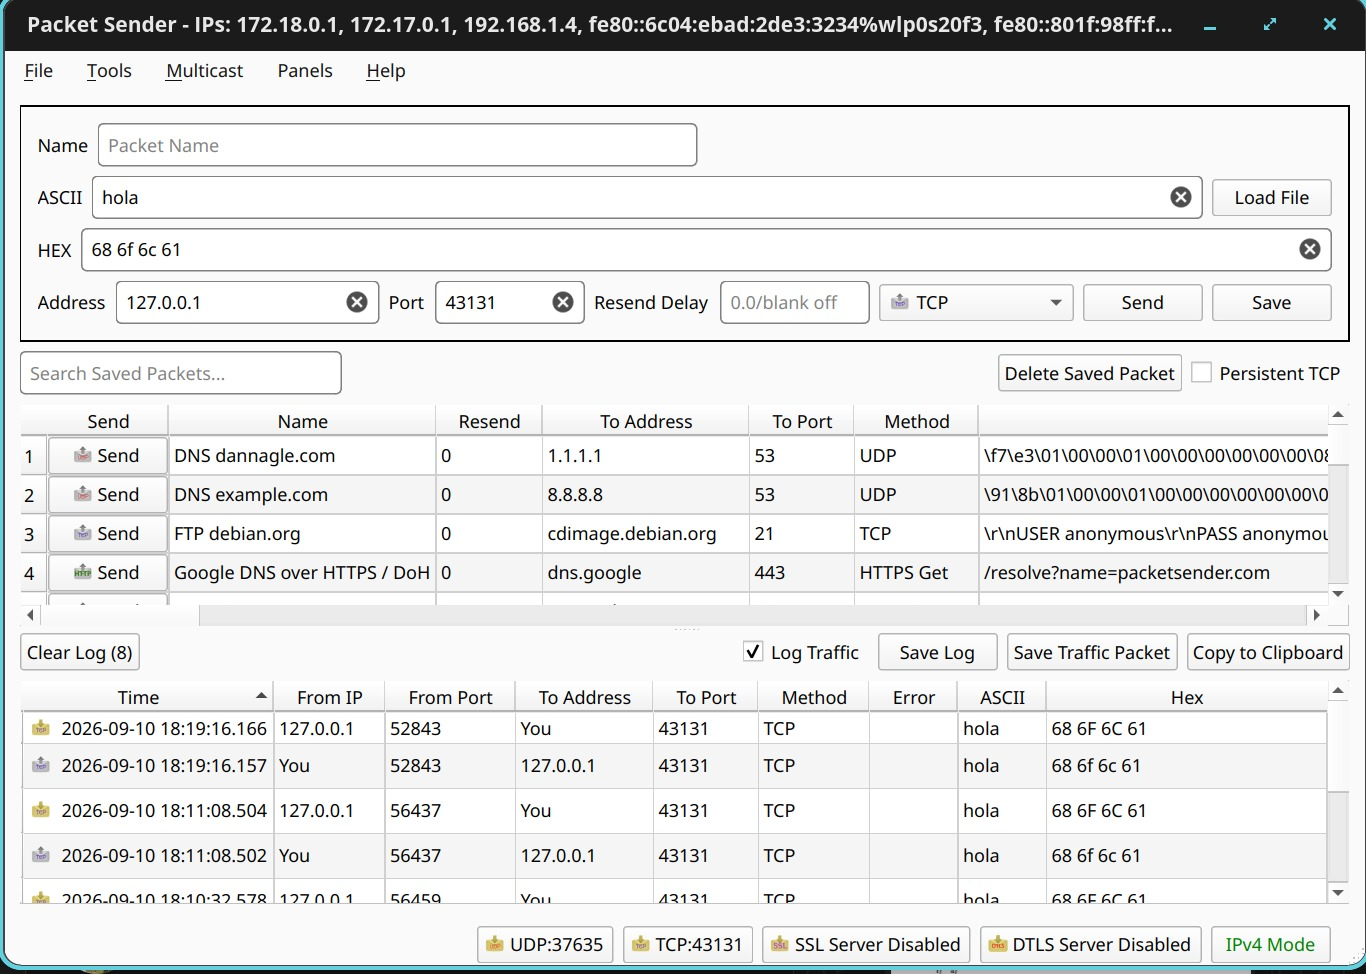
\includegraphics[width=0.6\linewidth,height=0.25\textheight,keepaspectratio]{punto_3_c.jpeg}
        \end{center}
Análisis de la captura de Packet Sender (Servidor y Cliente TCP Local). Configuración del Servidor TCP: Se observa el botón TCP:43131 indicando que la instancia de Packet Sender se encuentra escuchando tráfico en el puerto local 43131.
Configuración del Cliente TCP: Se definió la dirección de destino 127.0.0.1 (interfaz Loopback/localhost), el puerto 43131, el protocolo TCP y la carga útil en ASCII "hola" (representada en hexadecimal como 68 6f 6c 61).
        \item \leavevmode
        \begin{center}
            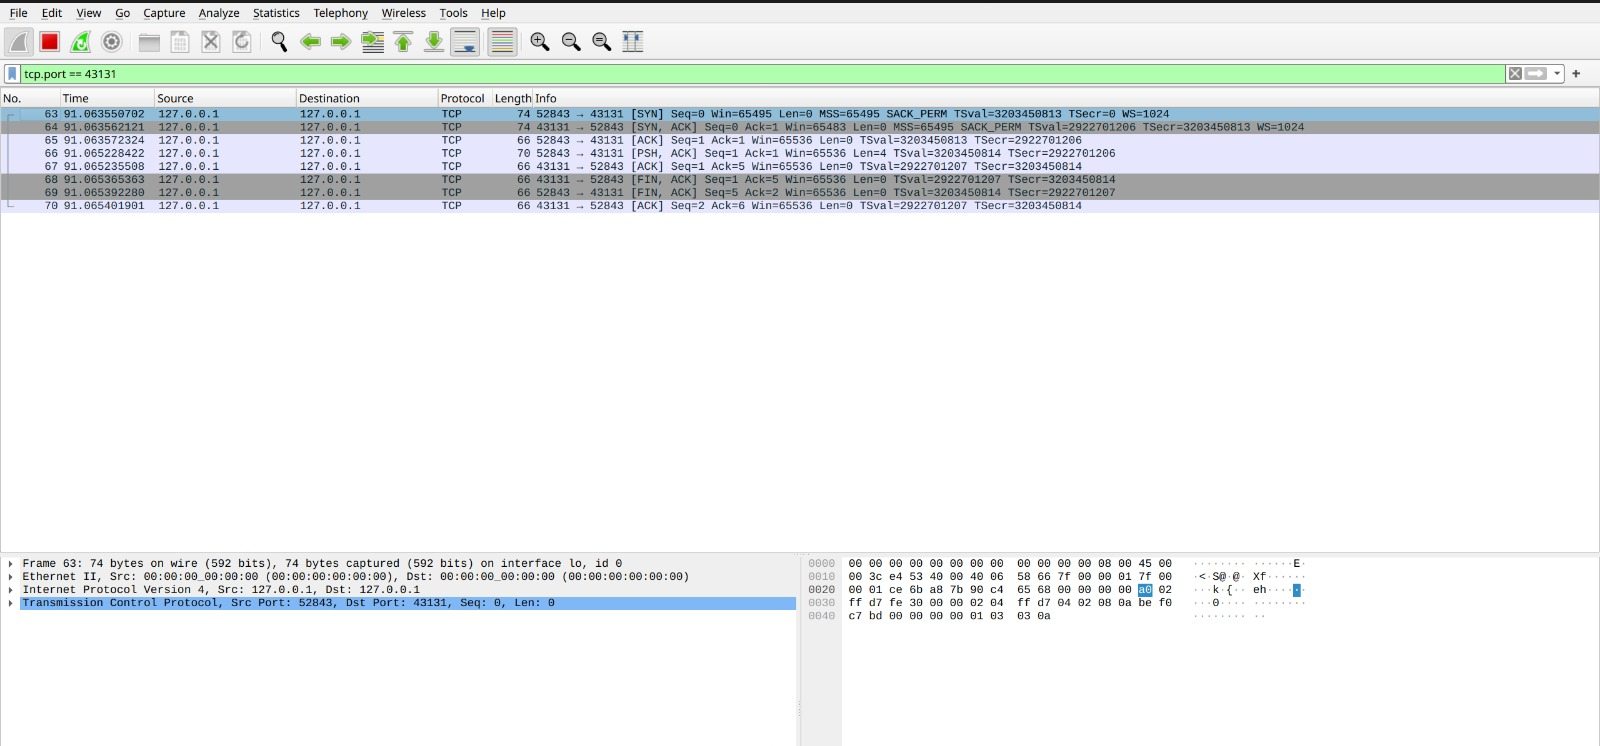
\includegraphics[width=0.8\linewidth,height=0.3\textheight,keepaspectratio]{punto_3_d.jpeg}
        \end{center}
        Análisis de la captura del Handshake e inspección del Payload (Paquete PSH, ACK)(Incluir aquí la captura de pantalla de Wireshark con el filtro tcp.port == 43131)Identificación de fases en Wireshark:Paso 1 (Handshake): Se observan los primeros tres paquetes intercambiados ([SYN], [SYN, ACK] y [ACK]) entre la dirección local 127.0.0.1 y el puerto asignado.Paso 2 (Payload): El paquete subsiguiente corresponde a la transmisión de datos y contiene los flags [PSH, ACK]. El flag PSH (Push) le indica a la pila de red que entregue los datos inmediatamente a la aplicación sin esperar a que el búfer se llene.Inspección del mensaje enviado: Al seleccionar el paquete [PSH, ACK] e inspeccionar la sección inferior (Data / Hex Bytes), se visualizan exactamente los bytes 68 6f 6c 61 en hexadecimal, los cuales corresponden a la cadena de caracteres ASCII "hola" configurada en Packet Sender
        \item \leavevmode
        \begin{center}
            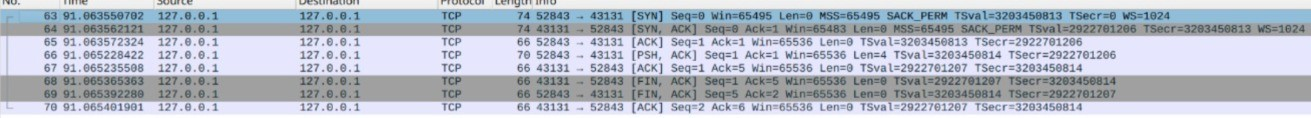
\includegraphics[width=0.8\linewidth,height=0.3\textheight,keepaspectratio]{punto_3_e_2.jpeg}
        \end{center}
        Al apagar el servidor o finalizar la sesión desde Packet Sender, se capturan en Wireshark los paquetes de terminación TCP. Se observan los flags [FIN, ACK] enviados para indicar el fin de la transmisión y sus correspondientes respuestas de confirmación [ACK], liberando formalmente los recursos de los sockets locales asignados a la comunicación.
        \item 
        Luego de analizar la captura del paquete de datos (PSH, ACK), se evidencia que el contenido enviado ("hola") es completamente visible en el panel hexadecimal de Wireshark sin requerir ningún proceso de descifrado.
Esto demuestra que el protocolo TCP en la capa de transporte garantiza la entrega ordenada y confiable de los segmentos, pero no proporciona asi ningún servicio de confidencialidad ni cifrado de la información. Ante esto un atacante en la misma red local que capture el tráfico puede leer íntegramente la información transmitida. Por esto, para mitigar esta vulnerabilidad, es fundamental implementar protocolos de seguridad sobre TCP en la capa de aplicación, tales como TLS/SSL (ejemplos: HTTPS o SSH).
    \end{enumerate}
    \item 
\end{enumerate}
\end{document}
